\documentclass[a4paper,12 pt]{report}
\usepackage[T1]{fontenc}
\usepackage[utf8]{inputenc}
\usepackage{lmodern}
\usepackage{listings}
\usepackage{graphicx}
\usepackage{float}
\usepackage{subcaption}
\usepackage{hyperref}
\usepackage{wrapfig}


%% STILE LISTINGS

\usepackage{xcolor}

\definecolor{codegreen}{rgb}{0,0.6,0}
\definecolor{codegray}{rgb}{0.5,0.5,0.5}
\definecolor{codepurple}{rgb}{0.58,0,0.82}
\definecolor{backcolour}{rgb}{0.95,0.95,0.92}

\lstdefinestyle{mystyle}{
    backgroundcolor=\color{backcolour},   
    commentstyle=\color{codegreen},
    keywordstyle=\color{magenta},
    numberstyle=\tiny\color{codegray},
    stringstyle=\color{codepurple},
    basicstyle=\ttfamily\footnotesize,
    breakatwhitespace=false,         
    breaklines=true,                 
    captionpos=b,                    
    keepspaces=true,                 
    numbers=left,                    
    numbersep=5pt,                  
    showspaces=false,                
    showstringspaces=false,
    showtabs=false,                  
    tabsize=2
}

\lstset{style=mystyle}

%% -----


% Resetta la numerazione dei chapter quando
% una nuova part viene creata
\makeatletter
\@addtoreset{chapter}{part}
\makeatother

% Rimuove l'indentazione quando si crea un nuovo paragrafo
\setlength{\parindent}{0pt}

\begin{document}
\tableofcontents

%%TODO: definire prima pagina

\documentclass[answers, 12 pt]{exam}

\usepackage[italian]{babel}
\usepackage{graphicx}
\usepackage[utf8]{inputenc}

%% links
\usepackage{hyperref}
\hypersetup{
	colorlinks=true,
	linkcolor=blue,
	filecolor=magenta,      
	urlcolor=cyan,
	pdftitle={\titolo},
	pdfpagemode=FullScreen,
}

\graphicspath{ {./img/} }


%% configurazione per i listing di codice
\usepackage{xcolor}
\usepackage{listings}
\colorlet{mycoolgray}{gray!40}

\lstdefinestyle{output}{
	numbers=none, % where to put the line-numbers
	numberstyle=\tiny, % the size of the fonts that are used for the line-numbers     
	backgroundcolor=\color{darkgray},
	basicstyle=\ttfamily\color{white},
	captionpos=b, % sets the caption-position to bottom
	breaklines=true, % sets automatic line breaking
	breakatwhitespace=false, 
}

\lstdefinestyle{cmd}{
	numbers=none, % where to put the line-numbers
	numberstyle=\tiny, % the size of the fonts that are used for the line-numbers     
	backgroundcolor=\color{mycoolgray},
	basicstyle=\ttfamily\color{black},
	captionpos=b, % sets the caption-position to bottom
	breaklines=true, % sets automatic line breaking
	breakatwhitespace=false, 
}
\title{Titolo della relazione} %% inserire qui il titolo della relazione 
\begin{document}
    \newcommand{\union}[2]{\underset{#1}\bigcup #2}
\newcommand{\inter}[2]{\underset{#1}\bigcap #2}

%% Compila questi campi !!

\newcommand{\esame}{Esame HPC}
\newcommand{\titolo}{Esercitazione 1 - Fedoraman}
\newcommand{\prof}{Osvaldo Gervasi}
\newcommand{\studente}{Nicolo' Vescera}
    % Thesis frontmatter --------------------------------------------

\thispagestyle{empty} %suppress page number

	\noindent % just to prevent indentation narrowing the line width for this line
	
\includegraphics[width=0.15\textwidth]{img/logoUniPg}
	\begin{minipage}[b]{0.7\textwidth}
		\centering
		{\Large{\textsc{Universit{\`a} di Perugia}}}\\
		\vspace{0.4 em}
		{\large {Dipartimento di Matematica e Informatica}}
		\vspace{0.6 em}
	\end{minipage}%
	
\includegraphics[width=0.15\textwidth]{img/logoDMI}
	
	\vspace{8 em}

	\begin{center}
		

	
		{\Huge{Appunti Knowledge Representation and Automated Reasoning }}\\
		\vspace{2 em}
		{\large { Autore: Chiara Luchini}}\\
		\vspace{5 em}
		{\large {Basati su:}}\\
		{\large {- Slides del Prof. Stefano Bistarelli}}\\
		{\large {- Lezioni del Prof. Stefano Bistarelli}}\\
		%{\large \textcolor{blu_dmi}{- Appunti lezioni online Prof. Alfredo Navarra}}\\
		
	
	

%		\makebox[380pt][c]{\textcolor{blu_dmi}{\textit{Advisor} \hfill \textit{}}}
%		\makebox[380pt][c]{\textcolor{blu_dmi}{\textbf{Dott. Francesco Santini \hfill}}}
		
		\vspace{6 em}
		\vfill
		
	{\rule{380pt}{.4pt}}\\
		\vspace{1.2 em}
		\large{{Anno Accademico 2021/2022}}
		
		
		
		
	\end{center}

% ------------------------------------------------------------------
    \newpage

    \section{Obbiettivo}

L'obiettivo di questa esercitazione \`{e}  quello di realizzare un cluster di 2 nodi nel quale si dovrà avere \textit{Pacemaker} come Cluster Resource Manager (\textit{CRM}), \textit{Corosync} come \textit{Cluster Engine}, \textit{Apache} come \textit{Web Server} e \textit{DRBD} per creare una risorsa replicata in tutti i nodi del cluster (\textit{Distributed Replicated Storage System}).

\section{Ambiente di Lavoro}

Questa esercitazione \`{e} stata svolta all'interno del seguente ambiente di lavoro:

\begin{itemize}
	\item \textbf{Hardware}: 
		\begin{itemize}
			\item \textbf{CPU}: AMD Ryzen 9 5900x
			\item \textbf{RAM}: 32 GB DDR4 @3200 MHz
		\end{itemize}
	\item \textbf{Software}:
		\begin{itemize}
			\item \textbf{Host OS:} Arch Linux
			\item \textbf{Guest OS}: Fedora 34 Server
			\item \textbf{Virtualization Software}: VirtualBox 6.1
		\end{itemize}
\end{itemize}

\section{Configurazione Macchine}

Per questa esercitazione sono necessarie 2 macchine virtuali che saranno i due nodi del nostro cluster. Ogni macchina \`{e} stata configurata come segue:

\begin{itemize}
	\item \textbf{Cores:} 5 Core
	\item \textbf{RAM:} 5GB
	\item \textbf{Dischi di archiviazione:}
		\begin{itemize}
			\item Disco Principale da 25 GB
			\item Disco per risorsa condivisa da 1 GB
		\end{itemize}
	\item \textbf{Scheda di Rete:} Scheda di rete con Bridge
\end{itemize}

\`{E} consigliato configurare una sola macchina, installare e configurare il sistema operativo e i software necessari, per poi utilizzare la funzione 'Clona' di VirtualBox per generare una copia identica senza dover ripetere tali operazioni nuovamente. Durante la fase di clonazione della macchina \`{e} necessario selezionare l'opzione "Generare nuovi Mac Address per ogni Network Adapter" come policy per la gestione dei Mac Address.

\begin{center}
	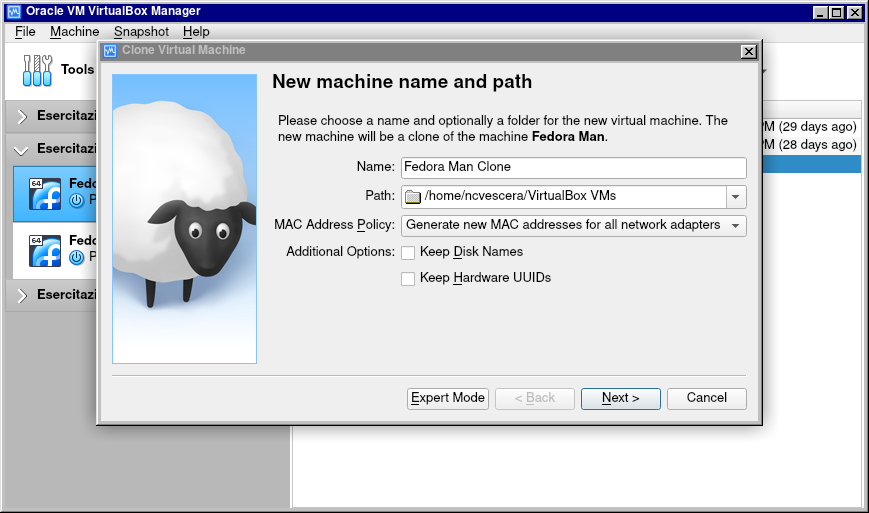
\includegraphics[scale=0.4]{screens/vb_macpolicy.png}
\end{center}
 
\section{Configurazione Software}

%% forse ci posso aggiungere una breve introduzione ...

\subsection{Sistema Operativo}

Qui ci va uno speghino un po dettagliato di come ho installato il sistema operativo. Piu immagini che altro, deve essere una brevissima guida.

Notare come di default il servizio sshd e' attivo e ho utilizzato ssh per connettermi e modificare le macchine

\subsection{Software Necessario}

Appena ho terminato la fase precendete ho provveduto ad aggiornare il sistema con il seguente comando, per evitare probelmi di compatibilit\`{a} e software obsoleto:

\begin{lstlisting}[style=cmd]
	sudo dnf -y upgrade
\end{lstlisting} 
\ \\
Poi ho installato i pacchetti necessari (\textit{Pacemaker}, \textit{Corosync}, \textit{Apache} e \textit{DRBD}) con: 

\begin{lstlisting}[style=cmd]
	sudo dnf -y install pacemaker corosync pcs
	sudo dnf -y install drbd-pacemaker drbd-udev
	sudo dnf -y install httpd
	sudo dnf -y install iptables-services
\end{lstlisting} 

\subsection{IP}

Per questa tipologia di esercitazione \`{e} buona norma assegnare IP statici alle macchine, ma nel mio caso non \`{e} stato necessario in quanto ho configurato il dhcp all'interno del mio router in modo da assegnare sempre lo stesso IP ai vari dispositivi della rete (dhcp statico).\\ %% ricontrollare affermazione di dhcp statico
Riporto per chiarezza la procedura per assegnare un IP statico all'interno di Fedora.

\begin{lstlisting}[style=cmd]
 sudo nmcli connection modify enp0s3 IPv4.address <ip>/24
 sudo nmcli connection modify enp0s3 IPv4.gateway <gateway>
 sudo nmcli connection modify enp0s3 IPv4.dns 8.8.8.8
 sudo nmcli connection modify enp0s3 IPv4.method manual
\end{lstlisting}
\ \\
Con il primo comando andiamo ad impostare l'ip della nostra macchina, \`{e} importate notare che bisogna sostituire \lstinline[style=cmd]|<ip>| con l'ip che vogliamo assegnare: e.g \lstinline[style=cmd]|192.168.178.32|.\\
Con il secondo configureremo l'indirizzo del gateway ed anche qui dobbiamo rimpiazzare \lstinline[style=cmd]|<gateway>| con il corretto ip: e.g. \lstinline[style=cmd]|192.168.178.1|.\\
\ \\
Per rendere effettive le modifiche basta riavviare il sistema.\\
Si pu\`{o} controllare il successo di questa operazione analizzando l'output del comando \lstinline[style=cmd]|route -n|, se restituisce qualcosa vuol dire che il tutto \`{e} andato a buon fine.

\subsection{\lstinline[style=cmd]|/etc/hosts| e \lstinline[style=cmd]|/etc/hostname|}

Ho modificato il file \lstinline[style=cmd]|/etc/hostname| definendo un nome diverso per ogni macchina dato che il mio router, tramite un servizio dns, mi permette di accedere alle macchine senza utilizzare il loro ip ma tramite il loro nome.

\begin{itemize}
	\item Nome Macchina 1: fedoraman
	\item Nome Macchina 2: fedoragirl
\end{itemize}
\ \\
In entrambe le macchine, alla fine del file \lstinline[style=cmd]|/etc/hosts| ho aggiunto le seguenti righe per facilitare poi la configurazione degli altri servizi (sostituendo \lstinline[style=cmd]|<ip macchina 1>| e \lstinline[style=cmd]|<ip macchina 2>| con i relativi ip):

\begin{lstlisting}[style=cmd]
 <ip macchina 1> Fedoraman
 <ip macchina 2> Fedoragirl
\end{lstlisting}

\subsection{AAA}

Prova di codice/output

\begin{lstlisting}[style=cmd]
:: There are 12 members in group texlive-most:
:: Repository extra
1) texlive-bibtexextra  2) texlive-core  3) texlive-fontsextra
4) texlive-formatsextra  5) texlive-games  6) texlive-humanities
7) texlive-latexextra  8) texlive-music  9) texlive-pictures
10) texlive-pstricks  11) texlive-publishers  12) texlive-science

Enter a selection (default=all): 
warning: texlive-core-2021.58710-2 is up to date -- reinstalling
resolving dependencies...
looking for conflicting packages...

Packages (13) perl-file-which-1.24-2  texlive-bibtexextra-2021.58697-1
texlive-core-2021.58710-2  texlive-fontsextra-2021.58704-1
texlive-formatsextra-2021.57972-1  texlive-games-2021.56833-1
texlive-humanities-2021.58589-1  texlive-latexextra-2021.58668-2
texlive-music-2021.58331-1  texlive-pictures-2021.58558-1
texlive-pstricks-2021.58293-1  texlive-publishers-2021.58683-1
texlive-science-2021.58667-1

Total Download Size:    629.40 MiB
Total Installed Size:  2116.49 MiB
Net Upgrade Size:      1728.35 MiB

:: Proceed with installation? [Y/n] 

\end{lstlisting}

\subsection{Parte 3}

\begin{lstlisting}[style=output]
:: There are 12 members in group texlive-most:
:: Repository extra
1) texlive-bibtexextra  2) texlive-core  3) texlive-fontsextra
4) texlive-formatsextra  5) texlive-games  6) texlive-humanities
7) texlive-latexextra  8) texlive-music  9) texlive-pictures
10) texlive-pstricks  11) texlive-publishers  12) texlive-science

Enter a selection (default=all): 
warning: texlive-core-2021.58710-2 is up to date -- reinstalling
resolving dependencies...
looking for conflicting packages...

Packages (13) perl-file-which-1.24-2  texlive-bibtexextra-2021.58697-1
texlive-core-2021.58710-2  texlive-fontsextra-2021.58704-1
texlive-formatsextra-2021.57972-1  texlive-games-2021.56833-1
texlive-humanities-2021.58589-1  texlive-latexextra-2021.58668-2
texlive-music-2021.58331-1  texlive-pictures-2021.58558-1
texlive-pstricks-2021.58293-1  texlive-publishers-2021.58683-1
texlive-science-2021.58667-1

Total Download Size:    629.40 MiB
Total Installed Size:  2116.49 MiB
Net Upgrade Size:      1728.35 MiB

:: Proceed with installation? [Y/n] 
\end{lstlisting}
\end{document}
\documentclass[answers, 12 pt]{exam}

\usepackage[italian]{babel}
\usepackage{graphicx}
\usepackage[utf8]{inputenc}

%% links
\usepackage{hyperref}
\hypersetup{
	colorlinks=true,
	linkcolor=blue,
	filecolor=magenta,      
	urlcolor=cyan,
	pdftitle={\titolo},
	pdfpagemode=FullScreen,
}

\graphicspath{ {./img/} }


%% configurazione per i listing di codice
\usepackage{xcolor}
\usepackage{listings}
\colorlet{mycoolgray}{gray!40}

\lstdefinestyle{output}{
	numbers=none, % where to put the line-numbers
	numberstyle=\tiny, % the size of the fonts that are used for the line-numbers     
	backgroundcolor=\color{darkgray},
	basicstyle=\ttfamily\color{white},
	captionpos=b, % sets the caption-position to bottom
	breaklines=true, % sets automatic line breaking
	breakatwhitespace=false, 
}

\lstdefinestyle{cmd}{
	numbers=none, % where to put the line-numbers
	numberstyle=\tiny, % the size of the fonts that are used for the line-numbers     
	backgroundcolor=\color{mycoolgray},
	basicstyle=\ttfamily\color{black},
	captionpos=b, % sets the caption-position to bottom
	breaklines=true, % sets automatic line breaking
	breakatwhitespace=false, 
}
\title{Titolo della relazione} %% inserire qui il titolo della relazione 
\begin{document}
    \newcommand{\union}[2]{\underset{#1}\bigcup #2}
\newcommand{\inter}[2]{\underset{#1}\bigcap #2}

%% Compila questi campi !!

\newcommand{\esame}{Esame HPC}
\newcommand{\titolo}{Esercitazione 1 - Fedoraman}
\newcommand{\prof}{Osvaldo Gervasi}
\newcommand{\studente}{Nicolo' Vescera}
    % Thesis frontmatter --------------------------------------------

\thispagestyle{empty} %suppress page number

	\noindent % just to prevent indentation narrowing the line width for this line
	
\includegraphics[width=0.15\textwidth]{img/logoUniPg}
	\begin{minipage}[b]{0.7\textwidth}
		\centering
		{\Large{\textsc{Universit{\`a} di Perugia}}}\\
		\vspace{0.4 em}
		{\large {Dipartimento di Matematica e Informatica}}
		\vspace{0.6 em}
	\end{minipage}%
	
\includegraphics[width=0.15\textwidth]{img/logoDMI}
	
	\vspace{8 em}

	\begin{center}
		

	
		{\Huge{Appunti Knowledge Representation and Automated Reasoning }}\\
		\vspace{2 em}
		{\large { Autore: Chiara Luchini}}\\
		\vspace{5 em}
		{\large {Basati su:}}\\
		{\large {- Slides del Prof. Stefano Bistarelli}}\\
		{\large {- Lezioni del Prof. Stefano Bistarelli}}\\
		%{\large \textcolor{blu_dmi}{- Appunti lezioni online Prof. Alfredo Navarra}}\\
		
	
	

%		\makebox[380pt][c]{\textcolor{blu_dmi}{\textit{Advisor} \hfill \textit{}}}
%		\makebox[380pt][c]{\textcolor{blu_dmi}{\textbf{Dott. Francesco Santini \hfill}}}
		
		\vspace{6 em}
		\vfill
		
	{\rule{380pt}{.4pt}}\\
		\vspace{1.2 em}
		\large{{Anno Accademico 2021/2022}}
		
		
		
		
	\end{center}

% ------------------------------------------------------------------
    \newpage

    \section{Obbiettivo}

L'obiettivo di questa esercitazione \`{e}  quello di realizzare un cluster di 2 nodi nel quale si dovrà avere \textit{Pacemaker} come Cluster Resource Manager (\textit{CRM}), \textit{Corosync} come \textit{Cluster Engine}, \textit{Apache} come \textit{Web Server} e \textit{DRBD} per creare una risorsa replicata in tutti i nodi del cluster (\textit{Distributed Replicated Storage System}).

\section{Ambiente di Lavoro}

Questa esercitazione \`{e} stata svolta all'interno del seguente ambiente di lavoro:

\begin{itemize}
	\item \textbf{Hardware}: 
		\begin{itemize}
			\item \textbf{CPU}: AMD Ryzen 9 5900x
			\item \textbf{RAM}: 32 GB DDR4 @3200 MHz
		\end{itemize}
	\item \textbf{Software}:
		\begin{itemize}
			\item \textbf{Host OS:} Arch Linux
			\item \textbf{Guest OS}: Fedora 34 Server
			\item \textbf{Virtualization Software}: VirtualBox 6.1
		\end{itemize}
\end{itemize}

\section{Configurazione Macchine}

Per questa esercitazione sono necessarie 2 macchine virtuali che saranno i due nodi del nostro cluster. Ogni macchina \`{e} stata configurata come segue:

\begin{itemize}
	\item \textbf{Cores:} 5 Core
	\item \textbf{RAM:} 5GB
	\item \textbf{Dischi di archiviazione:}
		\begin{itemize}
			\item Disco Principale da 25 GB
			\item Disco per risorsa condivisa da 1 GB
		\end{itemize}
	\item \textbf{Scheda di Rete:} Scheda di rete con Bridge
\end{itemize}

\`{E} consigliato configurare una sola macchina, installare e configurare il sistema operativo e i software necessari, per poi utilizzare la funzione 'Clona' di VirtualBox per generare una copia identica senza dover ripetere tali operazioni nuovamente. Durante la fase di clonazione della macchina \`{e} necessario selezionare l'opzione "Generare nuovi Mac Address per ogni Network Adapter" come policy per la gestione dei Mac Address.

\begin{center}
	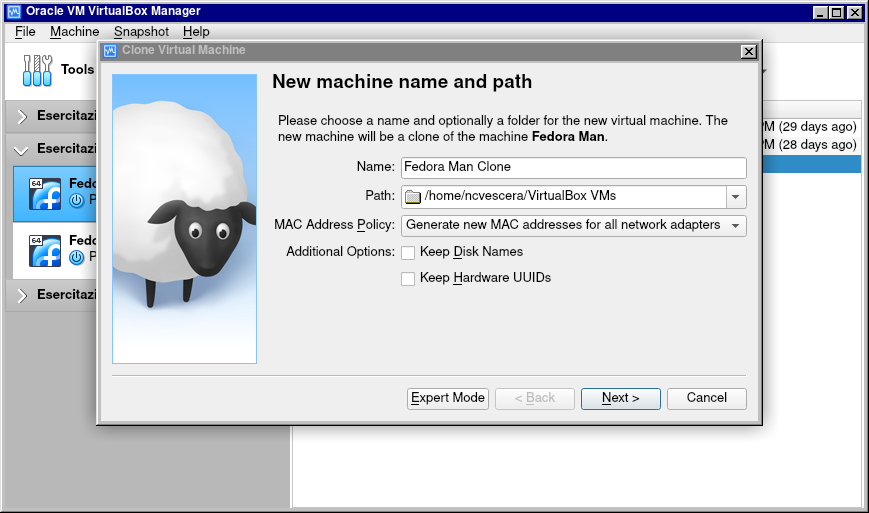
\includegraphics[scale=0.4]{screens/vb_macpolicy.png}
\end{center}
 
\section{Configurazione Software}

%% forse ci posso aggiungere una breve introduzione ...

\subsection{Sistema Operativo}

Qui ci va uno speghino un po dettagliato di come ho installato il sistema operativo. Piu immagini che altro, deve essere una brevissima guida.

Notare come di default il servizio sshd e' attivo e ho utilizzato ssh per connettermi e modificare le macchine

\subsection{Software Necessario}

Appena ho terminato la fase precendete ho provveduto ad aggiornare il sistema con il seguente comando, per evitare probelmi di compatibilit\`{a} e software obsoleto:

\begin{lstlisting}[style=cmd]
	sudo dnf -y upgrade
\end{lstlisting} 
\ \\
Poi ho installato i pacchetti necessari (\textit{Pacemaker}, \textit{Corosync}, \textit{Apache} e \textit{DRBD}) con: 

\begin{lstlisting}[style=cmd]
	sudo dnf -y install pacemaker corosync pcs
	sudo dnf -y install drbd-pacemaker drbd-udev
	sudo dnf -y install httpd
	sudo dnf -y install iptables-services
\end{lstlisting} 

\subsection{IP}

Per questa tipologia di esercitazione \`{e} buona norma assegnare IP statici alle macchine, ma nel mio caso non \`{e} stato necessario in quanto ho configurato il dhcp all'interno del mio router in modo da assegnare sempre lo stesso IP ai vari dispositivi della rete (dhcp statico).\\ %% ricontrollare affermazione di dhcp statico
Riporto per chiarezza la procedura per assegnare un IP statico all'interno di Fedora.

\begin{lstlisting}[style=cmd]
 sudo nmcli connection modify enp0s3 IPv4.address <ip>/24
 sudo nmcli connection modify enp0s3 IPv4.gateway <gateway>
 sudo nmcli connection modify enp0s3 IPv4.dns 8.8.8.8
 sudo nmcli connection modify enp0s3 IPv4.method manual
\end{lstlisting}
\ \\
Con il primo comando andiamo ad impostare l'ip della nostra macchina, \`{e} importate notare che bisogna sostituire \lstinline[style=cmd]|<ip>| con l'ip che vogliamo assegnare: e.g \lstinline[style=cmd]|192.168.178.32|.\\
Con il secondo configureremo l'indirizzo del gateway ed anche qui dobbiamo rimpiazzare \lstinline[style=cmd]|<gateway>| con il corretto ip: e.g. \lstinline[style=cmd]|192.168.178.1|.\\
\ \\
Per rendere effettive le modifiche basta riavviare il sistema.\\
Si pu\`{o} controllare il successo di questa operazione analizzando l'output del comando \lstinline[style=cmd]|route -n|, se restituisce qualcosa vuol dire che il tutto \`{e} andato a buon fine.

\subsection{\lstinline[style=cmd]|/etc/hosts| e \lstinline[style=cmd]|/etc/hostname|}

Ho modificato il file \lstinline[style=cmd]|/etc/hostname| definendo un nome diverso per ogni macchina dato che il mio router, tramite un servizio dns, mi permette di accedere alle macchine senza utilizzare il loro ip ma tramite il loro nome.

\begin{itemize}
	\item Nome Macchina 1: fedoraman
	\item Nome Macchina 2: fedoragirl
\end{itemize}
\ \\
In entrambe le macchine, alla fine del file \lstinline[style=cmd]|/etc/hosts| ho aggiunto le seguenti righe per facilitare poi la configurazione degli altri servizi (sostituendo \lstinline[style=cmd]|<ip macchina 1>| e \lstinline[style=cmd]|<ip macchina 2>| con i relativi ip):

\begin{lstlisting}[style=cmd]
 <ip macchina 1> Fedoraman
 <ip macchina 2> Fedoragirl
\end{lstlisting}

\subsection{AAA}

Prova di codice/output

\begin{lstlisting}[style=cmd]
:: There are 12 members in group texlive-most:
:: Repository extra
1) texlive-bibtexextra  2) texlive-core  3) texlive-fontsextra
4) texlive-formatsextra  5) texlive-games  6) texlive-humanities
7) texlive-latexextra  8) texlive-music  9) texlive-pictures
10) texlive-pstricks  11) texlive-publishers  12) texlive-science

Enter a selection (default=all): 
warning: texlive-core-2021.58710-2 is up to date -- reinstalling
resolving dependencies...
looking for conflicting packages...

Packages (13) perl-file-which-1.24-2  texlive-bibtexextra-2021.58697-1
texlive-core-2021.58710-2  texlive-fontsextra-2021.58704-1
texlive-formatsextra-2021.57972-1  texlive-games-2021.56833-1
texlive-humanities-2021.58589-1  texlive-latexextra-2021.58668-2
texlive-music-2021.58331-1  texlive-pictures-2021.58558-1
texlive-pstricks-2021.58293-1  texlive-publishers-2021.58683-1
texlive-science-2021.58667-1

Total Download Size:    629.40 MiB
Total Installed Size:  2116.49 MiB
Net Upgrade Size:      1728.35 MiB

:: Proceed with installation? [Y/n] 

\end{lstlisting}

\subsection{Parte 3}

\begin{lstlisting}[style=output]
:: There are 12 members in group texlive-most:
:: Repository extra
1) texlive-bibtexextra  2) texlive-core  3) texlive-fontsextra
4) texlive-formatsextra  5) texlive-games  6) texlive-humanities
7) texlive-latexextra  8) texlive-music  9) texlive-pictures
10) texlive-pstricks  11) texlive-publishers  12) texlive-science

Enter a selection (default=all): 
warning: texlive-core-2021.58710-2 is up to date -- reinstalling
resolving dependencies...
looking for conflicting packages...

Packages (13) perl-file-which-1.24-2  texlive-bibtexextra-2021.58697-1
texlive-core-2021.58710-2  texlive-fontsextra-2021.58704-1
texlive-formatsextra-2021.57972-1  texlive-games-2021.56833-1
texlive-humanities-2021.58589-1  texlive-latexextra-2021.58668-2
texlive-music-2021.58331-1  texlive-pictures-2021.58558-1
texlive-pstricks-2021.58293-1  texlive-publishers-2021.58683-1
texlive-science-2021.58667-1

Total Download Size:    629.40 MiB
Total Installed Size:  2116.49 MiB
Net Upgrade Size:      1728.35 MiB

:: Proceed with installation? [Y/n] 
\end{lstlisting}
\end{document}
\documentclass[answers, 12 pt]{exam}

\usepackage[italian]{babel}
\usepackage{graphicx}
\usepackage[utf8]{inputenc}

%% links
\usepackage{hyperref}
\hypersetup{
	colorlinks=true,
	linkcolor=blue,
	filecolor=magenta,      
	urlcolor=cyan,
	pdftitle={\titolo},
	pdfpagemode=FullScreen,
}

\graphicspath{ {./img/} }


%% configurazione per i listing di codice
\usepackage{xcolor}
\usepackage{listings}
\colorlet{mycoolgray}{gray!40}

\lstdefinestyle{output}{
	numbers=none, % where to put the line-numbers
	numberstyle=\tiny, % the size of the fonts that are used for the line-numbers     
	backgroundcolor=\color{darkgray},
	basicstyle=\ttfamily\color{white},
	captionpos=b, % sets the caption-position to bottom
	breaklines=true, % sets automatic line breaking
	breakatwhitespace=false, 
}

\lstdefinestyle{cmd}{
	numbers=none, % where to put the line-numbers
	numberstyle=\tiny, % the size of the fonts that are used for the line-numbers     
	backgroundcolor=\color{mycoolgray},
	basicstyle=\ttfamily\color{black},
	captionpos=b, % sets the caption-position to bottom
	breaklines=true, % sets automatic line breaking
	breakatwhitespace=false, 
}
\title{Titolo della relazione} %% inserire qui il titolo della relazione 
\begin{document}
    \newcommand{\union}[2]{\underset{#1}\bigcup #2}
\newcommand{\inter}[2]{\underset{#1}\bigcap #2}

%% Compila questi campi !!

\newcommand{\esame}{Esame HPC}
\newcommand{\titolo}{Esercitazione 1 - Fedoraman}
\newcommand{\prof}{Osvaldo Gervasi}
\newcommand{\studente}{Nicolo' Vescera}
    % Thesis frontmatter --------------------------------------------

\thispagestyle{empty} %suppress page number

	\noindent % just to prevent indentation narrowing the line width for this line
	
\includegraphics[width=0.15\textwidth]{img/logoUniPg}
	\begin{minipage}[b]{0.7\textwidth}
		\centering
		{\Large{\textsc{Universit{\`a} di Perugia}}}\\
		\vspace{0.4 em}
		{\large {Dipartimento di Matematica e Informatica}}
		\vspace{0.6 em}
	\end{minipage}%
	
\includegraphics[width=0.15\textwidth]{img/logoDMI}
	
	\vspace{8 em}

	\begin{center}
		

	
		{\Huge{Appunti Knowledge Representation and Automated Reasoning }}\\
		\vspace{2 em}
		{\large { Autore: Chiara Luchini}}\\
		\vspace{5 em}
		{\large {Basati su:}}\\
		{\large {- Slides del Prof. Stefano Bistarelli}}\\
		{\large {- Lezioni del Prof. Stefano Bistarelli}}\\
		%{\large \textcolor{blu_dmi}{- Appunti lezioni online Prof. Alfredo Navarra}}\\
		
	
	

%		\makebox[380pt][c]{\textcolor{blu_dmi}{\textit{Advisor} \hfill \textit{}}}
%		\makebox[380pt][c]{\textcolor{blu_dmi}{\textbf{Dott. Francesco Santini \hfill}}}
		
		\vspace{6 em}
		\vfill
		
	{\rule{380pt}{.4pt}}\\
		\vspace{1.2 em}
		\large{{Anno Accademico 2021/2022}}
		
		
		
		
	\end{center}

% ------------------------------------------------------------------
    \newpage

    \section{Obbiettivo}

L'obiettivo di questa esercitazione \`{e}  quello di realizzare un cluster di 2 nodi nel quale si dovrà avere \textit{Pacemaker} come Cluster Resource Manager (\textit{CRM}), \textit{Corosync} come \textit{Cluster Engine}, \textit{Apache} come \textit{Web Server} e \textit{DRBD} per creare una risorsa replicata in tutti i nodi del cluster (\textit{Distributed Replicated Storage System}).

\section{Ambiente di Lavoro}

Questa esercitazione \`{e} stata svolta all'interno del seguente ambiente di lavoro:

\begin{itemize}
	\item \textbf{Hardware}: 
		\begin{itemize}
			\item \textbf{CPU}: AMD Ryzen 9 5900x
			\item \textbf{RAM}: 32 GB DDR4 @3200 MHz
		\end{itemize}
	\item \textbf{Software}:
		\begin{itemize}
			\item \textbf{Host OS:} Arch Linux
			\item \textbf{Guest OS}: Fedora 34 Server
			\item \textbf{Virtualization Software}: VirtualBox 6.1
		\end{itemize}
\end{itemize}

\section{Configurazione Macchine}

Per questa esercitazione sono necessarie 2 macchine virtuali che saranno i due nodi del nostro cluster. Ogni macchina \`{e} stata configurata come segue:

\begin{itemize}
	\item \textbf{Cores:} 5 Core
	\item \textbf{RAM:} 5GB
	\item \textbf{Dischi di archiviazione:}
		\begin{itemize}
			\item Disco Principale da 25 GB
			\item Disco per risorsa condivisa da 1 GB
		\end{itemize}
	\item \textbf{Scheda di Rete:} Scheda di rete con Bridge
\end{itemize}

\`{E} consigliato configurare una sola macchina, installare e configurare il sistema operativo e i software necessari, per poi utilizzare la funzione 'Clona' di VirtualBox per generare una copia identica senza dover ripetere tali operazioni nuovamente. Durante la fase di clonazione della macchina \`{e} necessario selezionare l'opzione "Generare nuovi Mac Address per ogni Network Adapter" come policy per la gestione dei Mac Address.

\begin{center}
	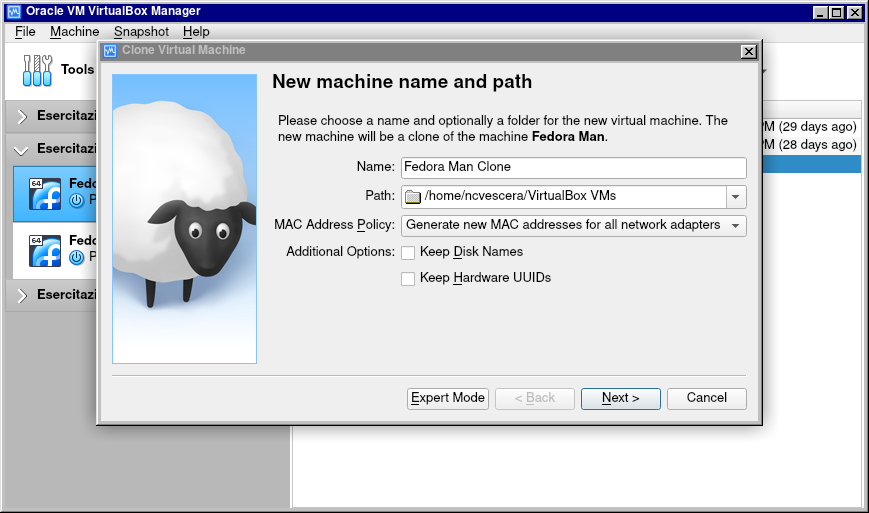
\includegraphics[scale=0.4]{screens/vb_macpolicy.png}
\end{center}
 
\section{Configurazione Software}

%% forse ci posso aggiungere una breve introduzione ...

\subsection{Sistema Operativo}

Qui ci va uno speghino un po dettagliato di come ho installato il sistema operativo. Piu immagini che altro, deve essere una brevissima guida.

Notare come di default il servizio sshd e' attivo e ho utilizzato ssh per connettermi e modificare le macchine

\subsection{Software Necessario}

Appena ho terminato la fase precendete ho provveduto ad aggiornare il sistema con il seguente comando, per evitare probelmi di compatibilit\`{a} e software obsoleto:

\begin{lstlisting}[style=cmd]
	sudo dnf -y upgrade
\end{lstlisting} 
\ \\
Poi ho installato i pacchetti necessari (\textit{Pacemaker}, \textit{Corosync}, \textit{Apache} e \textit{DRBD}) con: 

\begin{lstlisting}[style=cmd]
	sudo dnf -y install pacemaker corosync pcs
	sudo dnf -y install drbd-pacemaker drbd-udev
	sudo dnf -y install httpd
	sudo dnf -y install iptables-services
\end{lstlisting} 

\subsection{IP}

Per questa tipologia di esercitazione \`{e} buona norma assegnare IP statici alle macchine, ma nel mio caso non \`{e} stato necessario in quanto ho configurato il dhcp all'interno del mio router in modo da assegnare sempre lo stesso IP ai vari dispositivi della rete (dhcp statico).\\ %% ricontrollare affermazione di dhcp statico
Riporto per chiarezza la procedura per assegnare un IP statico all'interno di Fedora.

\begin{lstlisting}[style=cmd]
 sudo nmcli connection modify enp0s3 IPv4.address <ip>/24
 sudo nmcli connection modify enp0s3 IPv4.gateway <gateway>
 sudo nmcli connection modify enp0s3 IPv4.dns 8.8.8.8
 sudo nmcli connection modify enp0s3 IPv4.method manual
\end{lstlisting}
\ \\
Con il primo comando andiamo ad impostare l'ip della nostra macchina, \`{e} importate notare che bisogna sostituire \lstinline[style=cmd]|<ip>| con l'ip che vogliamo assegnare: e.g \lstinline[style=cmd]|192.168.178.32|.\\
Con il secondo configureremo l'indirizzo del gateway ed anche qui dobbiamo rimpiazzare \lstinline[style=cmd]|<gateway>| con il corretto ip: e.g. \lstinline[style=cmd]|192.168.178.1|.\\
\ \\
Per rendere effettive le modifiche basta riavviare il sistema.\\
Si pu\`{o} controllare il successo di questa operazione analizzando l'output del comando \lstinline[style=cmd]|route -n|, se restituisce qualcosa vuol dire che il tutto \`{e} andato a buon fine.

\subsection{\lstinline[style=cmd]|/etc/hosts| e \lstinline[style=cmd]|/etc/hostname|}

Ho modificato il file \lstinline[style=cmd]|/etc/hostname| definendo un nome diverso per ogni macchina dato che il mio router, tramite un servizio dns, mi permette di accedere alle macchine senza utilizzare il loro ip ma tramite il loro nome.

\begin{itemize}
	\item Nome Macchina 1: fedoraman
	\item Nome Macchina 2: fedoragirl
\end{itemize}
\ \\
In entrambe le macchine, alla fine del file \lstinline[style=cmd]|/etc/hosts| ho aggiunto le seguenti righe per facilitare poi la configurazione degli altri servizi (sostituendo \lstinline[style=cmd]|<ip macchina 1>| e \lstinline[style=cmd]|<ip macchina 2>| con i relativi ip):

\begin{lstlisting}[style=cmd]
 <ip macchina 1> Fedoraman
 <ip macchina 2> Fedoragirl
\end{lstlisting}

\subsection{AAA}

Prova di codice/output

\begin{lstlisting}[style=cmd]
:: There are 12 members in group texlive-most:
:: Repository extra
1) texlive-bibtexextra  2) texlive-core  3) texlive-fontsextra
4) texlive-formatsextra  5) texlive-games  6) texlive-humanities
7) texlive-latexextra  8) texlive-music  9) texlive-pictures
10) texlive-pstricks  11) texlive-publishers  12) texlive-science

Enter a selection (default=all): 
warning: texlive-core-2021.58710-2 is up to date -- reinstalling
resolving dependencies...
looking for conflicting packages...

Packages (13) perl-file-which-1.24-2  texlive-bibtexextra-2021.58697-1
texlive-core-2021.58710-2  texlive-fontsextra-2021.58704-1
texlive-formatsextra-2021.57972-1  texlive-games-2021.56833-1
texlive-humanities-2021.58589-1  texlive-latexextra-2021.58668-2
texlive-music-2021.58331-1  texlive-pictures-2021.58558-1
texlive-pstricks-2021.58293-1  texlive-publishers-2021.58683-1
texlive-science-2021.58667-1

Total Download Size:    629.40 MiB
Total Installed Size:  2116.49 MiB
Net Upgrade Size:      1728.35 MiB

:: Proceed with installation? [Y/n] 

\end{lstlisting}

\subsection{Parte 3}

\begin{lstlisting}[style=output]
:: There are 12 members in group texlive-most:
:: Repository extra
1) texlive-bibtexextra  2) texlive-core  3) texlive-fontsextra
4) texlive-formatsextra  5) texlive-games  6) texlive-humanities
7) texlive-latexextra  8) texlive-music  9) texlive-pictures
10) texlive-pstricks  11) texlive-publishers  12) texlive-science

Enter a selection (default=all): 
warning: texlive-core-2021.58710-2 is up to date -- reinstalling
resolving dependencies...
looking for conflicting packages...

Packages (13) perl-file-which-1.24-2  texlive-bibtexextra-2021.58697-1
texlive-core-2021.58710-2  texlive-fontsextra-2021.58704-1
texlive-formatsextra-2021.57972-1  texlive-games-2021.56833-1
texlive-humanities-2021.58589-1  texlive-latexextra-2021.58668-2
texlive-music-2021.58331-1  texlive-pictures-2021.58558-1
texlive-pstricks-2021.58293-1  texlive-publishers-2021.58683-1
texlive-science-2021.58667-1

Total Download Size:    629.40 MiB
Total Installed Size:  2116.49 MiB
Net Upgrade Size:      1728.35 MiB

:: Proceed with installation? [Y/n] 
\end{lstlisting}
\end{document}
\end{document}